\labeledsection{Statistical Learning}{sec:statistical_learning}
\anondefinition{
\defemph{Statistical Learning} has the goal to learn the correct \linkterm{probability distribution}{def:prob_distribution} of a \linkterm{random variable}{def:random_variable}
}{statistical_learning}

\Example{
\begin{itemize}
    \item Bayesian learning: learning probabilistic models (e.g. the \linkterm{CPD}{def:cond_prob_distribution} in \linkterm{Bayesian Networks}{def:bayes_net}) from observations.
    \item Maximum a Posteriori and Maximum Likelihood Learning
    \item \linkterm{Bayesian Networks}{def:bayes_net} Learning
\end{itemize}
}{}

\redbox{
We will discuss these topics but let's first explain the running example:
}

\Example{
\begin{figure}[H]
    \centering
    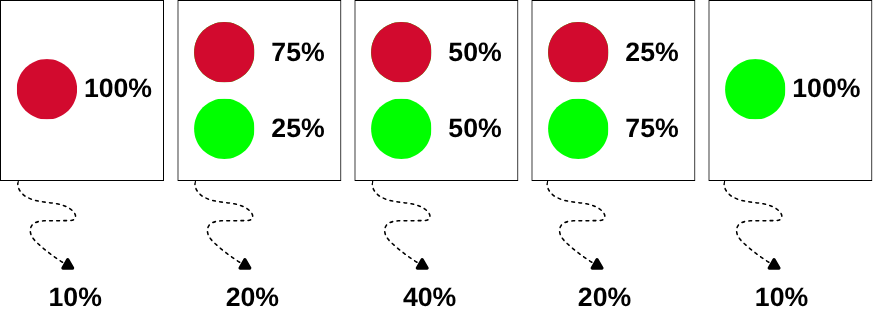
\includegraphics[width=0.6\linewidth]{images/candies.png}
\end{figure}

We have two flavors of candies, cherry and lime. We have five kinds of bags of candies where each kind contains different numbers of both flavors. 

We know that $10\%$ of our boxes contain only cherry candies, etc. We express that as \linkterm{priors}{def:bayesian_terms} of five \linkterm{hypotheses}{supervised_learning} $h_1 = 0.1, h_2=0.3, \cdots h_5 = 0.1$

We observed $10$ lime candies  drawn from some bag (which we do not know), we want to know what kind of bag it is and what flavor will the next candy be?

\textbf{Note: }every \linkterm{hypothesis}{supervised_learning} $h_i$ is itself a \linkterm{probability distribution}{def:prob_distribution} over the \linkterm{random variable}{def:random_variable} \textit{flavor}
}{candies_example}

Let $d_i$ be the event that the $i-$th drawn candy is green (lime), then the \linkterm{posterior}{def:bayesian_terms} of the \linkterm{hypotheses}{supervised_learning} keeps updating as $n$ increases for lime observations $\mathbf{d} =  d_{1:n}$:

\begin{figure}[H]
    \centering
    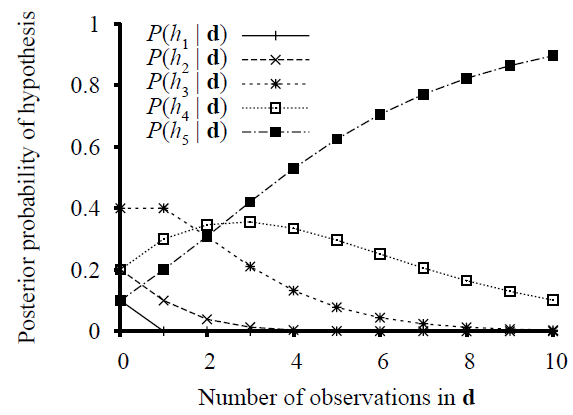
\includegraphics[width=0.6\linewidth]{images/candies_post.png}
\end{figure}

If the observations are \linkterm{IID}{def:iid}:
\[
P(d \mid h_i) = \prod_{j} P(d_j \mid h_i)
\]

\titledbox{Remember}{
\linkterm{likelihood}{def:bayesian_terms} $P(B \mid A)$ is the probability that the evidence $B$ would be observed if the hypothesis $A$ were true. (\Defref{def:bayesian_terms})
}

The \linkterm{likelihood}{def:bayesian_terms} of our observation $\mathbf{d} = d_{1:10}$ (10 lime candies) under each hypothesis $h_i$ is calculated as:
\begin{align*}
P(\mathbf{d} \mid h_1) &= (0.0)^{10} = 0 \\ 
P(\mathbf{d} \mid h_2) &= (0.25)^{10} = \frac{1}{1,048,576} \approx 9.54 \times 10^{-7} \\
P(\mathbf{d} \mid h_3) &= (0.5)^{10} = \frac{1}{1,024} \approx 9.77 \times 10^{-4} \\ 
P(\mathbf{d} \mid h_4) &= (0.75)^{10} = \frac{59,049}{1,048,576} \approx 0.0563 \\
P(\mathbf{d} \mid h_5) &= (1.0)^{10} = 1 
\end{align*}


The \linkterm{posterior}{def:bayesian_terms} probabilities originate from the hypothesis \linkterm{priors}{def:bayesian_terms} and are dynamically updated as data is observed.

\questionbox{
What is the probability that the $n+1$ candy is lime? 
}

\answerbox{
We compute the \linkterm{expected value}{expected_value} of the probability of the next candy being lime over all \linkterm{hypotheses}{supervised_learning}
\begin{align*}
P(d_{n+1} = \text{lime} \mid \mathbf{d}) 
&= \sum_{i} P(d_{n+1} = \text{lime} \land h_i \mid \mathbf{d}) \\
&= \sum_{i} \frac{P(d_{n+1} = \text{lime} \land h_i \land \mathbf{d})}{P(\mathbf{d})} \\
&= \sum_{i} \frac{P(d_{n+1} = \text{lime} \mid h_i, \mathbf{d}) \cdot P(h_i \land \mathbf{d})}{P(\mathbf{d})} \\
&= \sum_{i} P(d_{n+1} = \text{lime} \mid h_i, \mathbf{d}) \cdot \frac{P(h_i \land \mathbf{d})}{P(\mathbf{d})} \\
&= \sum_{i} P(d_{n+1} = \text{lime} \mid h_i, \mathbf{d}) \cdot P(h_i \mid \mathbf{d}) \\
&= \sum_{i} P(d_{n+1} = \text{lime} \mid h_i) \cdot P(h_i \mid \mathbf{d}) 
\end{align*}
}

We obtain the following predictions for different numbers of observed limes:
\begin{figure}[H]
    \centering
    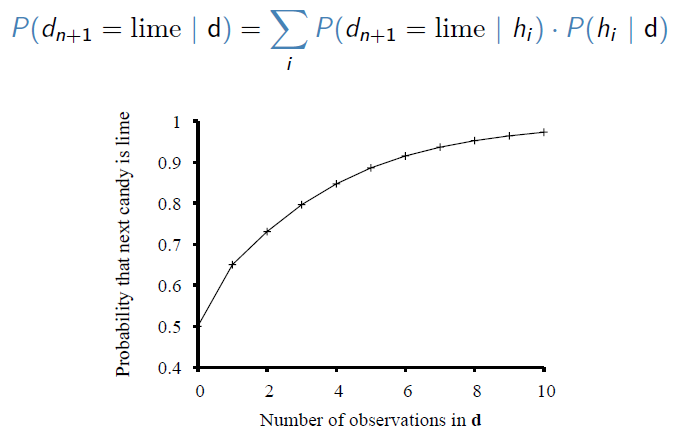
\includegraphics[width=0.6\linewidth]{images/candies_predictions.png}
\end{figure}

\anondefinition{
\defemph{Bayesian Learning} calculates the probability of each \linkterm{hypothesis}{supervised_learning} and makes predictions based on this
\begin{itemize}
    \item Given the data so far, each \linkterm{hypothesis}{supervised_learning} has a \linkterm{posterior}{def:bayesian_terms} probability:
    \[
        P(h_i \mid d) = \alpha (P(d \mid h_i) \cdot P(h_i))    
    \]
    where $P(d \mid h_i)$ is called the \linkterm{likelihood}{def:bayesian_terms} of the data under $h_i$ and $P(h_i)$ the \linkterm{hypothesis}{supervised_learning} \linkterm{prior}{def:bayesian_terms}
    \item \defemph{Bayesian Predictions} uses a \linkterm{likelihood}{def:bayesian_terms}-weighted average over the \linkterm{hypotheses}{supervised_learning}:
    \[
    \probd{X \mid d} := \sum_{i} \probd{X \mid h_i} \cdot P(h_i \mid d)
    \]
\end{itemize}
}{Bayesian_Learning}



\problembox{
Summing over the \linkterm{hypotheses space}{supervised_learning} is often interactable
}

\solutionbox{
Approximate the learning methods to simplify
}

\ideabox{
Make predictions w.r.t the \textit{"most probable"} \linkterm{hypothesis}{supervised_learning}
}

\anondefinition{
We call a \linkterm{hypothesis}{supervised_learning} $h_i$ that maximizes $P(h_i \mid d)$ a \defemph{Maximum a Posteriori (MAP) hypothesis} and refer to it as $h_{\text{MAP}}$
}{MAP_hyp}

\anondefinition{
\defemph{Maximum a Posteriori (MAP) Learning} chooses the \linkterm{MAP Hypthesis}{MAP_hyp}
}{MAP_learning}

\observationbox{
Predictions made according to a \linkterm{MAP hypothesis $h_{\text{MAP}}$}{MAP_hyp} are approximately \linkterm{Bayesian}{Bayesian_Learning} to the extent that $\probd{X \mid d} \approx \probd{X \mid h_{\text{MAP}}}$
}

\Example{
In our candy example, \linkterm{$h_{\text{MAP}}$}{MAP_hyp} = 5 after three limes in a row 
\begin{itemize}
    \item a \linkterm{MAP learner}{MAP_learning} would predict that candy $4$ is lime with probability of $1$
    \item \linkterm{Full Bayesian Learning}{Bayesian_Learning} would predict that of $0.8$ (see prediction curve)
\end{itemize}
}{}

\commandnote{
As more data arrive, the \linkterm{MAP}{MAP_learning} and \linkterm{Bayesian}{Bayesian_Learning} predictions become closer, because the competitors to the \linkterm{MAP hypothesis $h_{\text{MAP}}$}{MAP_hyp} become less and less probable.
}

\redbox{
Finding \linkterm{MAP hypotheses}{MAP_hyp} is often much easier than \linkterm{Bayesian Learning}{Bayesian_Learning}, because it requires solving an optimization problem instead of a large summation (or integration) problem
}

\titledbox{$\log$ Trick}{
Maximizing $P(h_i \mid d)$ means maximizing the product $P(d \mid h_i) \cdot P(h_i)$. To maximize that, we can maximize 
\[
\log_2 (P(d \mid h_i) \cdot P(h_i))
\]


$\leadsto$ maximizing the summation $\log_2 P(d \mid h_i) + \log_2 P(h_i)$
}

\titledbox{Minimization Trick}{
Instead of maximizing $\log_2 P(d \mid h_i) + \log_2 P(h_i)$ we can minimize:
\[
- \log_2 P(d \mid h_i) - \log_2 P(h_i)
\]
}

\anondefinition{
Let $x$ be a specific outcome of a \linkterm{random variable}{def:random_variable} $X$ with probability $P(X=x)$. The \defemph{self-information} (also called \defemph{information content} or \defemph{Shannon information}) of $x$ is:
\[
I(x) := -\log_2(P(x))
\]
}{self_information}

\titledbox{Sounds familiar?}{
The relationship between \linkterm{individual self-information}{self_information} $I(x)$ and the  \linkterm{total entropy}{entropy} $I(\tuple{p_1, \cdots, p_n})$ of a \linkterm{probability distribution}{def:prob_distribution} is that \linkterm{entropy}{entropy} is the \linkterm{expected value}{expected_value} (weighted average) of the \linkterm{self-information}{self_information} across all possible outcomes.

If we substitute the \linkterm{self-information}{self_information} of a single outcome, $I(x_i) = -\log_2(p_i)$, into the definition of \linkterm{entropy}{entropy}, we see this connection directly:

\[
I(\tuple{p_1, \cdots, p_n}) = \sum_{i=1}^{n} p_i \cdot \underbrace{\left(-\log_2(p_i)\right)}_{\text{Self-Information } I(x_i)} = \mathbb{E}[I(X)]
\]
}

\paragraph{Context in Learning:}
\begin{itemize}
    \item \textbf{Self-Information ($-\log_2(p)$):} Quantifies the cost or "surprise" of a single specific event. In MAP learning, we minimize the individual self-information of our specific data and hypothesis to find the shortest description length for our concrete sample.
    \item \textbf{Entropy ($\sum -p_i \log_2(p_i)$):} Quantifies the average uncertainty of the entire system. It represents the theoretical limit on the average number of bits required to encode arbitrary messages sent from that distribution.
\end{itemize}

\todo{
Delete this and write the thing in slide. And try to paraphrase it properly
}

